\documentclass[12pt,aspectratio=169,dvipsnames]{beamer}
\input{../mybeamer}

\usetikzlibrary{decorations.pathmorphing,patterns}

\title{Classes 1 and 2: Thermodynamics}
\subtitle{AP Physics 2}
\input{../me}
\input{../mycommands}


\begin{document}

\begin{frame}
  \maketitle
\end{frame}

\begin{frame}
  \centering
  {\LARGE\textbf{WELCOME TO AP PHYSICS 2}}
\end{frame}



\section{Temperature}

\begin{frame}{Temperature}
  \textbf{Temperature} is:
  \begin{itemize}
  \item a measure of the ``coldness''/''hotness'' of an object
  \item more accurately, a measure of the average
    \textbf{internal energy} of an object. (We will be defining that energy
    in our discussion)
  \end{itemize}
\end{frame}



\begin{frame}{Thermometric Properties}
  A \textbf{thermometric property} of an object are the physical properties
  that change with temperature. For example:
  \begin{itemize}
  \item Electrical resistance of a copper wire
  \item The length of an iron rod
  \item The volume taken up by mercury
  \item Pressure exerted by a gas
  \end{itemize}

  \vspace{.2in}An object is in a \textbf{thermal equilibrium} when
  \begin{itemize}
  \item thermometric properties are no longer changing
  \item heat is transferred in and out of the object at the same rate
  %\item has the same temperature as its surroundings
  \end{itemize}
\end{frame}



\begin{frame}{Zeroth Law of Thermodynamics}
  \textbf{Zeroth law of thermodynamics:} If two thermodynamic systems are each
  in thermal equilibrium with a third, then they are in thermal equilibrium
  with each other.
  \begin{itemize}
  \item Two objects $A$ and $B$ are in thermal equilibrium if the
    temperatures of the objects are the same
  \item Equal amounts of heat (energy) are flowing from $A$ to $B$ and from
    $B$ to $A$
  \item Establishes temperature as a measurement of heat, and allows us to
    define temperature scales
  \end{itemize}
  \begin{center}
    \pic{.22}{thezero}
  \end{center}
\end{frame}



\begin{frame}{Celsius Temperature Scale}
  For water, there are two equilibrium conditions that occur at atmospheric
  pressure consistently:
  \begin{itemize}
  \item\textbf{Ice point} (or \textbf{normal freezing/melting point}) where
    water and ice exist at this temperature in thermal equilibrium
  \item\textbf{Vapour point} (or \textbf{normal boiling point}) where water and
    water vapour exist in thermal equilibrium
  \end{itemize}
  In the \textbf{Celsius scale}, \SI0{\celsius} is the ice point, and
  \SI{100}{\celsius} is the vapour point\footnote{Fun fact: When Celsius
  first proposed the scale, the ice point was defined as \SI{100}{\celsius}
  while the vapour point was defined as \SI0\celsius. This means that the
  number gets bigger as it gets colder. But within a year or so, it was changed
  to the current scale}
\end{frame}



\section{Thermal Expansion}

\begin{frame}{Thermal Expansion}
  When temperature $T$ of an object with length $L$ increases, the object
  \emph{usually} expands. The \emph{thermal strain} ($\Delta L/L$) is
  proportional to the change in temperature ($\Delta T=T_f-T_i$) by the
  \textbf{coefficient of linear thermal expansion} ($\alpha$):
  
  \eq{-.1in}{
    \boxed{\frac{\Delta L}L\approx\alpha\Delta T}
  }
  \begin{center}
    \begin{tabular}{l|c|c}
      \rowcolor{pink}
      \textbf{Quantity} & \textbf{Symbol} & \textbf{SI Unit} \\ \hline
      Length & $L$ & \si\metre \\
      Change in length & $\Delta L$ & \si\metre \\
      Change in Temperature & $\Delta T$ & \si{\kelvin} or \si{\celsius}\\
      Coefficient of linear expansion & $\alpha$ & \si{\per\kelvin} or
      \si{\per\celsius}
    \end{tabular}
  \end{center}
  $\alpha$ is independent of pressure for solids and liquids, but may vary
  with $T$.
\end{frame}



\begin{frame}{Thermal Expansion}
  There is also a similar expression for \textbf{coefficient of volume
    expansion}:
  
  \eq{-.1in}{
    \boxed{\frac{\Delta V}V\approx\beta\Delta T}
  }

  $\beta$ is also independent of pressure for solids and liquids, but may vary
  with $T$.
  \begin{center}
    \begin{tabular}{l|c|c}
      \rowcolor{pink}
      \textbf{Quantity} & \textbf{Symbol} & \textbf{SI Unit} \\ \hline
      Volume      & $V$  & \si{\metre\cubed} \\
      Change in volume & $\Delta V$ & \si{\metre\cubed} \\
      Change in Temperature & $\Delta T$ & \si{\kelvin} or \si{\celsius}\\
      Coefficient of volume expansion & $\beta$ & \si{\per\kelvin}  or
      \si{\per\celsius}
    \end{tabular}
  \end{center}
  Careful application of calculus shows that for isotropic material (where
  $\alpha$ is the same in all direction):

  \eq{-.3in}{
    \beta = 3\alpha
  }
\end{frame}



\section{Ideal Gas Law}

\begin{frame}{Kinetic Theory of Gases}
  We begin the study of the thermodynamics of ideal gases using these
  assumptions:
  \begin{enumerate}
  \item The gas consists of a large number of identical molecules that are in
    high-speed random motion
  \item Molecular motion and interaction obey Newtonian laws of motion (i.e.\
    $\vec F_\text{net}=m\vec a$)
  \item Collision between molecules and with the walls of the container are
    \emph{elastic} (i.e.\ both momentum and kinetic energy are conserved)
  \item Molecules are separated, on average, by distances that are large
    compared to their diameters (i.e.\ the space occupied by the molecules are
    small compared to the space occupied by the gas as a whole)
  \item The only forces that the molecules experience are \emph{contact} forces
    (i.e.\ no gravitational, electrostatic forces on each other except when
    they collide)
  \end{enumerate}
\end{frame}



\begin{frame}{Random Motion}
  What does ``random motion'' mean in this case?
  \begin{itemize}
  \item Velocity vectors of all the gas molecules are different: some molecules
    move faster, some more slowly
  \item There is no preferred direction to the motion
  \item The average velocity of the gas molecules\footnote{This kind of average
  is called an ``ensemble average'', which will be discussed later} is zero
  \item The average \emph{speed} of the gas molecules is not zero (depends on
    temperature)
  \end{itemize}
\end{frame}


\begin{frame}{Volume of a Gas}
  \textbf{Volume} is the amount of space occupied by the gas, with an SI unit of
  \textbf{cubic metre} (\si{\metre\cubed}).
  \begin{center}
    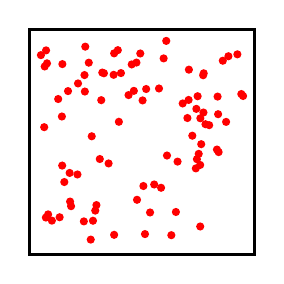
\begin{tikzpicture}[scale=1.3]
      \draw[very thick] (-.1,-.1) rectangle (2.1,2.1);
      \foreach \i in {1,...,90} \fill[red] (rand+1,rand+1) circle (.04);
    \end{tikzpicture}
  \end{center}
  The volume of a gas is \emph{not} the sum of the volumes of the individual
  atoms or molecules. Most of this occupied volume is empty space.
\end{frame}



\begin{frame}{Density of a Gas}
  The \textbf{density} is the ratio of the mass of the gas and the volume
  occupied by the gas:

  \eq{-.1in}{
    \boxed{
      \rho=\frac MV
    }
  }

  The SI unit of density is \textbf{kilogram per cubic metre}
  (\si{\kilo\gram\per\metre\cubed}).
  \begin{center}
    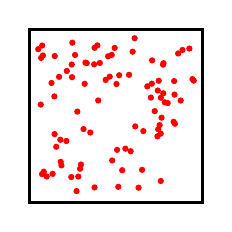
\begin{tikzpicture}
      \draw[very thick] (-.1,-.1) rectangle (2.1,2.1);
      \foreach \i in {1,...,90} \fill[red] (rand+1,rand+1) circle (.04);
    \end{tikzpicture}
  \end{center}
  For an ideal gas, the density is very low. (The reality is that no gas is
  truly ideal. However, the lower the density, the better the gas is
  approximated as an ideal gas. This is why helium is a very close to an
  ideal gas.)
  %The volume of a gas is \emph{not} the sum of the volumes of the individual
  %atoms. Most of this occupied volume is empty space.
\end{frame}



\begin{frame}{Pressure of a Gas}
  \begin{columns}
    \column{.7\textwidth}
    When gas molecules collide, they exert a force on each other and on the
    container. The \textbf{pressure} is that force $F$ that a gas exerts on the
    container, divided by the surface area of the container $A$ when the
    molecules collide with it:

    \eq{-.1in}{
      \boxed{
        P=\frac FA
      }
    }

    The SI unit of pressure is  \textbf{pascal} (\si\pascal) where

    \eq{-.15in}{
      \SI1\pascal=\SI1{\newton\per\metre\squared}
    }

    \vspace{-.2in}At thermal equilibrium, pressure is evenly distributed in the
    gas

    \column{.3\textwidth}
    \centering
    \begin{tikzpicture}[scale=1.3]
      \draw[very thick] (-.1,-.1) rectangle (2.1,2.1);
      \foreach \i in {1,...,90} \fill[red] (rand+1,rand+1) circle (.04);
      \foreach \xy in {.2,.4,...,1.8}{
        \begin{scope}[axes]
          \draw (.2,\xy)--(-.1,\xy);
          \draw (\xy,.2)--(\xy,-.1);
          \draw (1.8,\xy)--(2.1,\xy);
          \draw (\xy,1.8)--(\xy,2.1);
        \end{scope}
      }
    \end{tikzpicture}
  \end{columns}
\end{frame}



\begin{frame}{Absolute Temperature}
  William Thomson (a.k.a.\ Lord Kelvin) and James Joule discovered that when a
  gas is heated or cooled at \emph{constant volume}, there is a \emph{linear}
  relationship between pressure and temperature:
  \begin{center}
    \begin{tikzpicture}
      \begin{scope}[rotate=25,thick,OrangeRed]
        \draw[dashed] (0,0)--(1,0);
        \draw (1,0)--(5,0);
      \end{scope}
      \begin{scope}[rotate=32,thick,MidnightBlue]
        \draw[dashed] (0,0)--(1,0);
        \draw (1,0)--(5.2,0);
      \end{scope}
      \draw[axes] (0,0)--(5,0) node[right]{$T_C$};
      \draw[axes] (2,0)--(2,2.5) node[left]{$P$};
      \draw (0,0)--(0,-.15) node[below]{\SI{-273.15}\celsius};
    \end{tikzpicture}
  \end{center}
  Regardless of the type of gas, amount of gas, or the volume of gas, pressure
  is always zero at \SI{-273.15}\celsius. Since pressure cannot be negative;
  no temperature exists below that value.
\end{frame}



\begin{frame}{Absolute Temperature}
  The \textbf{absolute temperature} $T$ (or \textbf{thermodynamic temperature})
  is obtained by shifting the ``null point'' (where temperature is zero) from
  the Celsius temperature $T_C$.
  
  \eq{-.1in}{
    \boxed{T = T_C + 273.15}
  }
  \begin{itemize}
  \item A temperature of \SI0{\kelvin} is called
    \textbf{absolute zero} (Note that absolute zero is impossible to obtain
    because of quantum-mechanic effects, discussed in Class \#14)
  \item This scale is consistent with physical and thermodynamic properties
    of gases
  \item Note: the temperature \emph{change} of \SI1{\kelvin} is the same as
    \SI1\celsius, i.e.:

    \eq{-.1in}{
      \Delta T=\Delta T_C
    }
  \end{itemize}
\end{frame}
 


%\begin{frame}{Relationship Between Temperature and Pressure}
%  More accurately, the relationship between absolute temperature $T$ and
%  pressure $P$ of a gas at constant volume is defined using its triple point:
%
%  \eq{-.1in}{
%    T=\frac{T_\text{tp}}{P_\text{tp}}P
%  }
%
%  \textbf{Triple point} is a combination of pressure and temperature where the
%  solid, liquid and vapour phases of a substance may coexist in thermal
%  equilibrium.
%  \begin{itemize}
%  \item The triple point temperature for water is at
%    $T_\text{tp}=\SI{273.16}\kelvin$, or $\SI{.01}\celsius$
%  \item Triple point pressure for water is $P_\text{tp}=\SI{611.2}\pascal$
%  \end{itemize}
%\end{frame}




\begin{frame}{Ideal Gas Law for Low-Density Gases}
  Robert Boyle (1627-1691) discovered that, when a gas is allowed to expand or
  compress at \emph{constant temperature}, the product of pressure $P$ and $V$
  remain constant (\textbf{Boyle's law}):

  \eq{-.1in}{
    PV=\text{constant}
 }

  \vspace{-.15in}From the previous discussion on the absolute temperature scale,
  we also know that at \emph{constant volume}, temperature is proportional to
  pressure. Combining the two discoveries yields this equation:

  \eq{-.2in}{
    PV=CT
  }

  \vspace{-.15in}where ``C'' is some constant to be determined.
\end{frame}



\begin{frame}{Ideal Gas Law for Low-Density Gases}
  Thought experiment:
  \begin{itemize}
  \item Two identical containers with the same volume $V$, same amount of same
    kind of gas, at same pressure $P$ and same temperature $T$
  \item When the containers are combined and the molecules are free to move,
    $P$ and $T$ remain the same, but $V$ and $N$ both increases by factor of 2
  \end{itemize}
  Therefore $C$ must scale with the number of molecules $N$, which
  modifies the equation to the \textbf{ideal gas law}:

  \eq{-.1in}{
    \boxed{PV=Nk_BT}
  }

  The constant $k_B=\SI{1.381e-23}{\joule\per\kelvin}$ is called
  \textbf{Boltzmann's constant}. It is found experimentally to have the same
  value for any kind or amount of gas.
\end{frame}



\begin{frame}{Ideal Gas Law}
  The ideal gas law is often expressed in a different form in chemistry
  courses:  

  \eq{-.1in}{
    \boxed{PV=nRT}
  }

  \vspace{-.15in}where:
  \begin{itemize}
  \item $n=N/N_A$ is the number of moles of the gas
  \item $R=k_BN_A=\SI{8.314}{\kilo\gram\per\mol.\kelvin}$ is the
    \textbf{universal gas constant}, and
  \item $N_A=\num{6.022e23}$ is \textbf{Avogadro's number}, which is the number
    of molecules in one mole\footnote{One \emph{mole} of substance is the
    number of atoms in 12 grams of carbon-12 atoms. This number is also
    related to the definition of the \emph{unified atomic mass unit}, which
    will be discussed in the last topic of the course, on nuclear physics.} of
    the substance
  \end{itemize}
  The ideal gas law
  %is an \textbf{equation of state}, because it
  relates all the quantities that define the \emph{state} of a gas: pressure
  $P$, volume $V$ and temperature $T$. Both forms of the equations are used in
  AP Physics 2.
  \vspace{.2in}
\end{frame}



\section{Maxwell-Boltzmann Distribution}

\begin{frame}{Maxwell-Boltzmann Distribution}
  As gas molecules collide elastically with each other inside the
  container\footnote{Recall the discussion on elastic collision from AP
  Physics 1, or Physics 12, except for gases, collisions are not in one
  dimension (which are very easy) but in three dimensions.}:
  \begin{itemize}
  \item Some molecules \emph{gain} kinetic energy (therefore moving faster),
    while
  \item Some molecules \emph{lose} kinetic energy (therefore moving slower)
  \item Individual collisions are random occurrences (determined by
    probabilities), but
  \item The overall behaviour of the molecules at thermal equilibrium is very
    predictable
  \end{itemize}
\end{frame}



\begin{frame}{Maxwell-Boltzmann Distribution}
  At thermal equilibrium, the distribution of particle speeds $v$ for an ideal
  gas in a container at temperature $T$ is given by the
  \textbf{Maxwell-Boltzmann distribution} function:

  \eq{-.15in}{
    f(v,T)=4\pi\left[\frac m{2\pi k_BT}\right]^{\frac32}v^2
    \exp\left[-\frac{mv^2}{2k_BT}\right]
  }
  Note: $\exp(x)=e^x$
  \begin{center}
    \begin{tabular}{l|c|c}
      \rowcolor{pink}
      \textbf{Quantity} & \textbf{Symbol} & \textbf{SI Unit} \\ \hline
      Maxwell-Boltzmann dist.\ function & $f(v)$ &\si{\second\per\metre}\\
      Molecular mass       & $m$   & \si{\kilo\gram} \\
      Particle speed       & $v$   & \si{\metre\per\second} \\
      Absolute temperature & $T$   & \si\kelvin \\
      Boltzmann's constant & $k_B$ & \si{\joule\per\kelvin}
    \end{tabular}
  \end{center}
  AP Physics 2 is not concerned with the (very difficult) mathematics, only
  the overall concept, so you don't need to memorize this equation
\end{frame}



\begin{frame}{Maxwell-Boltzmann Distribution}
  \vspace{.15in}
  \begin{columns}
    \column{.45\textwidth}
    \pic{1.05}{maxwell-boltzmann}
    
    \column{.55\textwidth}
    \begin{itemize}
    \item This kind of function is called a \textbf{probability density
      function}
    \item The area under the distribution curve is 1 (all probabilities sums to
      \SI{100}\percent)
    \item The peak of the distribution shifts to higher speeds as $T$ increases
    \item The peak, which represents the most-probable speed $v_\text{prob}$,
      is lower at higher temperatures
    \end{itemize}
  \end{columns}
\end{frame}



\begin{frame}{Maxwell-Boltzmann Distribution}
  \begin{center}
    \pic{.5}{speed-distribution}
  \end{center}
  There are three particles speeds that are important: the most-probable speed
  $v_\text{prob}$, the mean (average) speed $\langle v \rangle$ and the
  root-mean-square speed $v_\text{rms}$.
\end{frame}



\begin{frame}{Most Probable Speed}
  \begin{columns}
    \column{.45\textwidth}
    \pic1{speed-distribution}
    
    \column{.55\textwidth}
    The \textbf{most probable speed} $v_\text{prob}$ is the peak (i.e.\ mode)
    of the distribution function. This is the speed you are most likely to find
    a molecule travelling at:

    \eq{-.05in}{
      v_\text{prob}=\sqrt{\frac{2k_BT}m}=\sqrt{\frac{2RT}M}
    }
  \end{columns}
  \vspace{-.05in}where $m$ is the molecular mass of the gas, $R$ is the
  universal gas constant, and $M$ is the molar mass\footnote{That is, the mass
  of 1 mole of the substance.}. $v_\text{prob}$ is obtained through using basic
  calculus\footnote{Albeit not necessarily simple. It involves finding the
  derivative of $f(v)$ and solving for $v$ where $f'(v)=0$.}. We can see that
  the most probable speed is proportional to the square root of absolute
  temperature:
  
  \eq{-.15in}{
    v_\text{prob}\propto\sqrt T
  }
\end{frame}



\begin{frame}{Mean/Average Speed}
  \begin{columns}
    \column{.45\textwidth}
    \pic1{speed-distribution}
    
    \column{.55\textwidth}
    The \textbf{mean speed} $\langle v\rangle$ (or \textbf{average speed}) is
    the arithmetic average of $N$ particles:
    
    \vspace{-.2in}{\large
      \begin{align*}
        \langle v\rangle &=\frac{v_1+v_2+\cdots+v_N}N\\
        &=\sqrt{\frac{8k_BT}{\pi m}}=\sqrt{\frac{8RT}{\pi M}}
      \end{align*}
    }
  \end{columns}
  The above value for $\langle v\rangle$ is obtained using basic integral
  calculus\footnote{The Maxwell-Boltzmann distribution function is continuous
  in $v$, so this is done by computing the integral
  $\langle v\rangle=\int_0^\infty vf(v)dv$. The Maxwell-Boltzmann distribution
  acts as a weighting function}. Like $v_\text{prob}$, $\langle v\rangle$ is
  also proportional to square root of absolute temperature:
  
  \eq{-.15in}{
    \langle v\rangle\propto\sqrt T
  }
\end{frame}



\begin{frame}{Side Note: Averaging}
  In AP Physics 1,
  %(or any physics course that you have previously taken),
  you have encountered two types of averaging:
  \begin{itemize}
  \item\textbf{Time averaging} (when the physical quantity of a
    \emph{single} object evolves over time). For example, average velocity,
    average acceleration (kinematics) and average force (momentum and impulse)
    are:

      \eq{-.13in}{
        \vec v_\text{avg}=\frac{\Delta\vec x}{\Delta t}\quad\quad
        \vec a_\text{avg}=\frac{\Delta\vec v}{\Delta t}\quad\quad
        \vec F_\text{avg}=\frac{\Delta\vec p}{\Delta t}
      }

    \item\textbf{Spatial averaging} (when the physical quantity of a
      \emph{single} object evolves over some distance). For example, the work
      done by the average force:
      
      \eq{-.13in}{
        F_\text{avg}=\frac W{\Delta x}
      }
  \end{itemize}
  Notice that there are \emph{two} definitions of average force. It is
  important to understand what kind of averaging we are doing
\end{frame}




\begin{frame}{Side Note: Ensemble Average}
  In this current example, the averaging is the arithmetic average amongst
  \emph{many} particles. This is known as an \textbf{ensemble average}. If
  there are $N$ particles, each with a physical property $X$, the ensemble
  average of $X$ (the notation is $\langle x\rangle$) is defined as:

  \eq{-.1in}{
    \langle x\rangle = \frac{X_1+X_2+\cdots+X_N}N=\frac{\sum_{i=1}^N X_i}N
  }

  For a large number of gas molecules, travelling with random motion, we
  care about the average speed ($\langle v\rangle$) and the average of the
  speed squared ($\langle v^2\rangle$)
\end{frame}




\begin{frame}{Root-Mean-Square (RMS) Speed}
  %\begin{center}
  %  \pic{.4}{speed-distribution}
  %\end{center}
  When studying ideal gases, we are \emph{most} interested in the average
  \emph{kinetic energy} $\langle K\rangle$ of the gas molecules, which scales
  with $v^2$. The average value of $v^2$ (i.e.\ $\langle v^2\rangle$) is
  therefore

  \vspace{-.15in}{\large
    \begin{align*}
      \langle K\rangle &=\dfrac{K_1+K_2+\cdots+K_N}N\\
      &=\dfrac{\frac12mv_1^2+\frac12mv_2^2+\cdots+\frac12mv_N^2}N
      =\frac12m
      \underbracket[1.3pt]{
        \left[\frac{v_1^2+v_2^2+\cdots+v_N^2}N\right]
      }_{\langle v^2\rangle}
    \end{align*}
  }
  
  Using ``basic'' integral calculus\footnote{This is accomplished by the
  integral $\langle v^2\rangle=\int_0^\infty v^2f(v)dv$. Again, the
  Maxwell-Boltzmann distribution function acts as a weighting function}, we can
  show that

  \eq{-.1in}{
    \langle v^2\rangle=\frac{3k_BT}m
  }
\end{frame}



\begin{frame}{Root-Mean-Square (RMS) Speed}
  The speed that gives the average kinetic energy is called the
  \textbf{root-mean-square speed} $v_\text{rms}$, which is the square root of
  $\langle v^2\rangle$:

  \eq{-.1in}{
    \underbracket[1.3pt]{v_\text{rms}=\sqrt{\langle v^2\rangle}}_{
      \text{i.e.\ }v_\text{rms}^2=\langle v^2\rangle}
    =\sqrt{\frac{3k_BT}m}=\sqrt{\frac{3RT}M}
  }

  ``Root mean square'' literally means ``the square root of the mean of the
  square''. Like $v_\text{prob}$ and $\langle v\rangle$, $v_\text{rms}$ is
  also proportional to the square root of absolute temperature:

  \eq{-.1in}{
    v_\text{rms}\propto\sqrt T
  }
\end{frame}



\begin{frame}{Average Kinetic Energy of an Ideal Gas}
  From the expression of $v_\text{rms}$, and relating to the average kinetic
  energy, it is easy to show the average kinetic energy of $N$ ideal-gas
  molecules is:
  
  \eq{-.1in}{
    \langle K \rangle=\frac12mv_\text{rms}^2=
    \frac12m\left[\sqrt{\frac{3k_BT}m}\right]^2
    \quad\rightarrow\quad
    \boxed{\langle K\rangle=\frac32k_BT}
  }

  The \emph{total} kinetic energy of an ideal gas therefore scales linearly
  with temperature:

  \eq{-.1in}{
    K_\text{total}=N\langle K\rangle=\frac32Nk_BT=\frac32nRT
  }
\end{frame}



\section{First Law of Thermodynamics}


\begin{frame}{Law of Conservation of Energy}
  In the law of conservation of energy\footnote{This is, perhaps, the most
  important concept in fundamental physics, and a major topic that is studied
  in AP Physics 1, as well as in Grade 11 \& 12 Physics}, the change in the
  total energy of a system $E_\text{sys}$ is equal to the net external
  mechanical work $W_\text{ext}$ done from outside the system:

  \eq{-.15in}{
    \boxed{
      \Delta E_\text{sys}=W_\text{ext}
    }
  }

  The \emph{consequence} of the law of conservation of energy is that, in an
  isolated system, energy cannot be created or destroyed; it can only change in
  form.
\end{frame}



\begin{frame}{Law of Conservation of Energy}
  In AP Physics 1, we learned that the total energy is the sum of all the
  kinetic and potential energies of the objects in the system, called
  \textbf{mechanical energy}.

  \eq{-.1in}{
    E_\text{sys} = \sum K +
    \underbracket[1pt]{ \sum U_g + \sum U_e + \cdots}_\text{potential energies}
  }

  Therefore, the \emph{change} in total energy is the total change in all the
  forms of energy:
  
  \eq{-.1in}{
    \Delta E_\text{sys} =
    \sum\Delta K + \sum\Delta U_g + \sum\Delta U_e + \cdots
  }


  \textbf{Question: But have we accounted for \emph{all} the energies in the
    system?}
\end{frame}



\begin{frame}[t]{Kinetic, Potential and Internal Energies}
  \begin{columns}[T]
    \column{.3\textwidth}
    \begin{tikzpicture}[scale=.75]
  \begin{scope}[thick]
    \draw (-1,5)--(3,5);
    \draw (-1,-4)--(3,-4) node[right]{\scriptsize$h=0$};
    \draw[dashed] (-1,2.8)--+(4,0) node[right]{\scriptsize Unstretched};
    \draw[decoration={aspect=.4, segment length=5, amplitude=6, coil},
      decorate] (1,5)--(1,2.1) node[midway,right=4]{$k$};
    \draw[vectors] (.5,2.8)--(.5,2.1) node[midway,left]{$\vec x$};
    \draw[fill=gray!10] (-.1,-.1) rectangle (2.1,2.1);
    \draw[vectors] (2.5,2)--(2.5,0) node[midway,right]{$\vec v$};
    \draw[|<-] (-.5,1)--(-.5,-4) node[midway,left]{$h$};
  \end{scope}
  \foreach \i in {1,...,90} \fill[red] (rand+1,rand+1) circle (.05);
\end{tikzpicture}


    \column{.7\textwidth}
    Consider a container of gas with a total mass $m$, oscillating from the
    ceiling. At the macroscopic level, the system has a total
    \textbf{mechanical energy} which includes:
    \begin{itemize}
    \item A \emph{bulk} kinetic energy of

      \eq{-.18in}{ K=\dfrac12 mv^2 }

    \item\vspace{-.1in}A gravitational potential energy of

      \eq{-.18in}{ U_g=mgh }

    \item\vspace{-.18in} An elastic potential energy of

      \eq{-.18in}{ U_e=\frac12kx^2 }
    \end{itemize}
    %The sum of these kinetic and potential energies is called the
    %\textbf{mechanical energy}.
  \end{columns}
\end{frame}



\begin{frame}[t]{Kinetic, Potential and Internal Energies}
  \begin{columns}[T]
    \column{.3\textwidth}
    \begin{tikzpicture}[scale=.75]
  \begin{scope}[thick]
    \draw (-1,5)--(3,5);
    \draw (-1,-4)--(3,-4) node[right]{\scriptsize$h=0$};
    \draw[dashed] (-1,2.8)--+(4,0) node[right]{\scriptsize Unstretched};
    \draw[decoration={aspect=.4, segment length=5, amplitude=6, coil},
      decorate] (1,5)--(1,2.1) node[midway,right=4]{$k$};
    \draw[vectors] (.5,2.8)--(.5,2.1) node[midway,left]{$\vec x$};
    \draw[fill=gray!10] (-.1,-.1) rectangle (2.1,2.1);
    \draw[vectors] (2.5,2)--(2.5,0) node[midway,right]{$\vec v$};
    \draw[|<-] (-.5,1)--(-.5,-4) node[midway,left]{$h$};
  \end{scope}
  \foreach \i in {1,...,90} \fill[red] (rand+1,rand+1) circle (.05);
\end{tikzpicture}


    \column{.7\textwidth}
    But the random motion of the air molecules also contribute to additional
    energy of the system, called the \textbf{internal energy}, or
    \textbf{thermal energy}, $E_\text{int}$ which is the sum of all their
    kinetic and potential energies at the \emph{microscopic} level:

    \eq{-.1in}{
      \boxed{ E_\text{int}=K_\text{micro} + U_\text{micro} }
    }

    Internal energy is a function of the molecules' absolute temperature.
  \end{columns}
\end{frame}



\begin{frame}{First Law of Thermodynamics}
  When applying the law of conservation of energy to a thermodynamic system:
  \begin{itemize}
  \item No change in bulk kinetic energy and potential energies (i.e.\ how
    fast the container moves, or how high it is above Earth, or how much the
    spring stretches, does not affect the temperature of the gas inside)
  \item The only energy change to the system is its internal energy
  \end{itemize}
  This reduces the equation to:
  
  \eq{-.1in}{
    \xcancel{\sum\Delta K} + \xcancel{\sum\Delta U} + \Delta E_\text{int}=
    W_\text{ext}
  }

  \textbf{HOWEVER}, aside from the (macroscopic) mechanical work done, there is
  also a ``non-mechanical'' transfer of energy (i.e.\ work done at the
  \emph{microscopic} level), called \textbf{heat} $Q$. The law of conservation
  of energy becomes the first law of thermodynamics:

  \eq{-.1in}{
    \Delta E_\text{int}= Q + W_\text{ext}
  }
\end{frame}



\begin{frame}{First Law of Thermodynamics}
  In the \textbf{first law of thermodynamics}\footnote{The equation is written
  in a \emph{slightly} different notation from the last slide by convention,
  in that here, we use ``$U$'' for internal energy instead of macroscopic
  potential energy},
  the change in internal energy of a thermodynamic system ($\Delta U$) is the
  sum of the heat transferred ($Q$) and the net external mechanical work ($W$)
  done \emph{to} the system\footnote{\textbf{IMPORTANT NOTE:} The equation is
  often written as $\Delta U=Q-W$, where $W$ is the work done \emph{by} the
  system. Since both conventions are commonly use, you must be very careful.}:
  
  \eq{-.1in}{
    \boxed{\Delta U=Q+W}
  }
  \begin{center}
    \begin{tabular}{l|c|c}
      \rowcolor{pink}
      \textbf{Quantity} & \textbf{Symbol} & \textbf{SI Unit} \\ \hline
      Change in internal energy of a system & $\Delta U$ & \si\joule \\
      Mechanical work done \emph{to} the system & $W$    & \si\joule \\
      Heat transfer into the system & $Q$ & \si\joule
    \end{tabular}
  \end{center}
  \vspace{.3in}
\end{frame}



\begin{frame}{Internal Energy}
  %As shown in an earlier slide,
  Internal energy {\color{OrangeRed}$U$} is the total kinetic \& potential
  energies of the molecules at the microscopic level.

  \eq{-.1in}{
    \boxed{\Delta\textcolor{OrangeRed}{U}=Q+W}
  }

  \vspace{-.05in}To calculate the internal energy of a collection of molecules,
  we first note the average kinetic energy of an ideal-gas molecule. A molecule
  can translate in 3 dimensions (its velocity can have the $\hat x$, $\hat y$
  and $\hat z$ components), so kinetic energy can be divided amongst the 3
  ``degrees of freedom'' (DoF):

  \vspace{-.2in}{\large
    \begin{align*}
      \langle K \rangle&=\frac12m\langle v^2\rangle
      =\frac12m\langle v_x^2+v_y^2+v_z^2\rangle\\
      &=\frac12m\langle v_x^2\rangle+\frac12m\langle v_y^2\rangle+
      \frac12m\langle v_z^2\rangle
    \end{align*}
  }
\end{frame}



\begin{frame}{Internal Energy}
  Since the motion of the molecules is random (i.e.\ no preferred direction of
  motion), the component averages must be the same, i.e.

  \eq{-.1in}{
    \langle v_x^2\rangle=\langle v_y^2\rangle=\langle v_z^2\rangle
  }

  \vspace{-.1in}\textbf{Equipartition theorem:} Since the motion is random, the
  internal energy of a thermodynamic system must be evenly divided between each
  DoF, and each DoF has a contribution of

  \eq{-.1in}{
    \frac12Nk_BT\quad\text{\normalsize or}\quad\frac12nRT
  }
  
  \vspace{-.1in}towards the total internal energy
\end{frame}



\begin{frame}{Internal Energy}
  \textbf{Monatomic or ideal gases} have 3 translational DoF. The internal
  energy is the total kinetic energy, shown a few slides ago:
  
  \eq{-.12in}{
    U=\frac32Nk_BT=\frac32nRT
  }

  \textbf{Diatomic gases}\footnote{In
  %\footnote{By definition, diatomic gases cannot also
  %be ideal gases. However, in
  AP Physics 2, you will often hear of a ``diatomic ideal gas''. In those
  cases, we assume an equality rather than an approximation} have 3
  translational DoF, and 2 rotational DoF, therefore the total internal energy
  is:
    
  \eq{-.2in}{
    U\approx\frac52Nk_BT\quad\text{\normalsize or}\quad
    U\approx\frac52nRT
  }
  \vspace{.2in}
\end{frame}



\begin{frame}{Internal Energy}
  \textbf{Solids} typically have 3 translational DoF, plus 3 vibrational DoF in
  elastic compression, and therefore the internal energy is:

  \eq{-.15in}{
    U\approx3Nk_BT\quad\text{\normalsize or}\quad 3nRT
  }

  \vspace{-.1in}The above approximation is more accurate for solids that have a
  well-defined lattice structures (e.g.\ metals and their alloys). For
  other substances, this approximation can be \emph{very} inaccurate

  \vspace{.2in}(What is conspicuously missing is the description of liquids.
  In general, there is no viable approximation for the internal energy of a
  liquid because of the complexity.)
\end{frame}


\begin{frame}{Internal Energy}
  Regardless of whether a substance is a gas, liquid or a solid, the internal
  energy is always proportional to absolute temperature:

  \eq{-.1in}{
    U\propto T
  }

  \vspace{-.1in}Therefore we can observe changes in the internal energy by
  measuring how (and by how much) temperature is changing
\end{frame}



\begin{frame}{Heat}
  \textbf{Heat} {\color{blue}$Q$} is the spontaneous non-mechanical transfer of
  energy \emph{into} the system, through conduction, convection and radiation.

  \eq{-.2in}{
    \boxed{\Delta U={\color{blue}Q}+W}
  }
  \begin{itemize}
  \item Heat transfer $Q$ is:
    \begin{itemize}
    \item $+$ if heat is added to the system
    \item $-$ if heat leaves the system
    \end{itemize}
  \item The net flow of energy is always from the higher temperature to low
    temperature (second law of thermodynamics)
  \item Two objects are in thermal equilibrium if the temperatures are the same
  \end{itemize}
\end{frame}



\begin{frame}{Mechanical Work}
  
  {\color{orange}$W$} is the mechanical work\footnote{The full
    definition in calculus form is $W=\int PdV$ (i.e.\ pressure times change in
    volume) which is derived from the definition of mechanical work:
    $W=\int\vec F\cdot d\vec x$ (force times distance)} done \emph{to}
  the system by the surrounding.

  \eq{-.1in}{
    \boxed{
      \Delta U=Q+{\color{orange}W}
    }
  }
  \begin{itemize}
  \item Work is done if the volume changes
  \item At constant pressure:

    \eq{-.15in}{
      W=-P\Delta V
    }
    
  \item\vspace{-.1in}\textbf{POSITIVE} if done \emph{to} the system, e.g.\
    pushing a piston to compress gas in an engine
  \item\textbf{NEGATIVE} if done \emph{by} the system, e.g.\ using steam
    pressure to push a piston or shaft
  \end{itemize}
  \vspace{.4in}
\end{frame}



%\begin{frame}{Example of a Thermal System}
%  \centering
%  \begin{tikzpicture}[scale=1.2]
%    \begin{scope}[thick]
%      \draw[fill=cyan!10] (5,0)--(1.5,0)--(1.5,1)--(0,1)--(0,2)--(4,2)
%      --(4,.7)--(5,.7);
%      \draw[fill=black!2] (.2,1.2) rectangle (1.5,1.8);
%    \end{scope}
%    \fill (4.8,0) rectangle (5,.7);
%
%    \node at (2.8,1.3) {\normalsize gas};
%    
%    \foreach \y in {.05,.25,...,.7} \draw[vectors] (5.5,\y)--(5,\y);
%    \node[right=4,text width=135,draw=black,fill=gray!10] at (5.5,.35){
%      {\scriptsize External pressure compressing the gas through the piston
%        does \emph{positive} work \emph{to} the thermal system\par}
%      
%      \vspace{-.38in}{\Large
%        \begin{displaymath}
%          +W
%        \end{displaymath}
%      }
%      
%      \vspace{-.07in}{\scriptsize Work done \emph{by} the system is
%        negative.\par}
%    };
%    \foreach \x in {1.75,2.25,...,4}
%    \draw[axes,red,decorate,decoration=snake] (\x,2.1)--+(0,1.2);
%    \node[above=4,text width=100,red,draw=red,fill=red!10] at (2.8,3.3){
%      {\scriptsize Heat loss through radiation at the walls of the container
%        \par}
%
%      \vspace{-.38in}{\Large
%        \begin{displaymath}
%          -Q
%        \end{displaymath}
%        \par}
%    };
%  \end{tikzpicture}
%\end{frame}



\section{Heat Capacity}

\begin{frame}{Heat Capacity}
  In many situations, heat transferred from a thermodynamic system ($Q$) can be
  directly related to the change in temperature ($\Delta T$) by the object's
  \textbf{heat capacity} ($C$):

  \eq{-.1in}{
    Q = C\Delta T
  }

  \vspace{-.1in}$C$ has a unit of \textbf{joule per kelvin}
  (\si{\joule\per\kelvin}) or \text{joule per degree Celsius}
  (\si{\joule\per\celsius}). Heat capacity depends on the object's mass as well
  as its composition.
%  It can be also expressed using a related quantity called the \textbf{molar
%    heat capacity}, which is the energy required to heat \SI1{\mol} of a
%  substance by \SI1\kelvin:
%
%  \eq{-.15in}{
%    \boxed{ Q = nc_m\Delta T }
%  }
  However, more practically, the \textbf{specific heat capacity} (lower case
  $c$) is the energy required to raise the temperature of \SI1{\kilo\gram} of
  a substance by \SI1{\kelvin} or \SI1\celsius:
  
  \eq{-.1in}{
    \boxed{Q = mc\Delta T}
  }

  $c$ is a physical property of a substance. The SI unit is
  \textbf{joule per kilogram per kelvin} (\si{\joule\per\kilo\gram.\kelvin})
\end{frame}



\begin{frame}{Specific Heat Capacity for Solids}
  For a solid, when heat is added or removed, little to no work is done
  \emph{by} the solid. Therefore all the heat goes into changing the internal
  energy:

  \eq{-.1in}{
    Q\approx\Delta U\approx\underbracket[1pt]{3nR}_{mc}\Delta T
  }

%  The molar heat capacity is approximately the same for \emph{most} solids.
%  Note that the universal gas constant still makes an appearance!
%
%  \eq{-.15in}{
%    c_m\approx\frac Cn=3R
%  }

  And the specific heat capacity can be obtained by:
  %$m=nM$ from the heat capacity:

  \eq{-.1in}{
    c\approx\frac{3nR}m\quad\rightarrow\quad c\approx\frac{3R}M
    %c\approx\frac Cm=\frac{3nR}{nM}\quad\rightarrow\quad c\approx\frac{3R}M
  }

  This approximation applies best to substances that have a well-defined
  lattice structure (e.g.\ metals), but may be \emph{very} inaccurate
  non-metallic substances. In general, $c$ is determined experimentally
\end{frame}



\begin{frame}{Heat Capacities for Gases at Constant Volume}
  For gases, the value for heat capacities depends on whether work is also
  done when heat is added/removed from the gas. When heat is added/removed at
  \emph{constant volume}, no work is done, therefore all the heat goes into
  changing the internal energy:

  \begin{itemize}
  \item For monatomic or ideal gases:
    
    \eq{-.1in}{
      Q=\Delta U={\color{magenta}\frac32nR}\Delta T=
      {\color{magenta}mc_v}\Delta T\quad\rightarrow\quad
      c_v=\frac{3nR}{2m}=\frac{3R}M
    }
    
  \item For diatomic gases:
    
    \eq{-.15in}{
      Q=\Delta U\approx{\color{cyan}\frac52nR}\Delta T
      ={\color{cyan}mc_v}\Delta T=\quad\rightarrow\quad
      c_v\approx\frac{5nR}{2m}=\frac{5R}{2M}
    }
  \end{itemize}
\end{frame}



%\begin{frame}{Heat Capacities of Gases at Constant Volume}
%%  The molar heat capacity of a gas is therefore:
%%
%%  \eq{-.1in}{
%%    c_m=\frac{C_v}n=\frac32R\quad\text{(ideal)}\quad\quad
%%    c_m=\frac{C_v}n\approx\frac52R\quad\text{(diatomic)}
%%  }
%
%  And the specific heat capacities for ideal/monatomic and diatomic gases are,
%  respectively:
%
%  \eq{-.1in}{
%    c_v=\frac{C_v}m=\frac32\frac RM\quad\text{(ideal)}\quad\quad
%    c_v=\frac{C_v}m\approx\frac52\frac RM\quad\text{(diatomic)}
%  }
%\end{frame}



\begin{frame}{Heat Capacities of Gases at Constant Pressure}
  When heat is added/removed at \emph{constant pressure}, volume changes,
  and work is done by/to the gas. This work can be related to temperature change
  using the ideal gas law:

  \eq{-.15in}{
    W=-P\Delta V = -nR\Delta T
  }
  
  \vspace{-.15in}The heat added is therefore

  \eq{-.15in}{
    Q=\Delta U - W =mc_v\Delta T + nR\Delta T\quad\rightarrow\quad
    \boxed{c_p=c_v+nR}
  }

%  which means that heat capacities are:
%
%  \eq{-.15in}{
%    C_p=\frac52nR\quad\text{(ideal)}\quad\quad
%    C_p\approx\frac72nR\quad\text{(diatomic)}
%  }
%\end{frame}
%
%
%
%\begin{frame}{Heat Capacities of Gases at Constant Pressure}
%  The molar heat capacity of a gas at constant pressure is therefore:
%
%  \eq{-.1in}{
%    c_m=\frac52R\quad\text{(ideal)}\quad\quad
%    c_m\approx\frac72R\quad\text{(diatomic)}
%  }

  which means that the specific heat capacity is:

  \eq{-.1in}{
    c_p=\frac52\frac RM\quad\text{(ideal)}\quad\quad
    c_p\approx\frac72\frac RM\quad\text{(diatomic)}
  }
\end{frame}



\begin{frame}{Specific Heat Capacity}
  \begin{columns}
    \column{.55\textwidth}
    The actual specific heat capacities of different substances are usually
    found experimentally

    \column{.45\textwidth}
    \centering
    \begin{tabular}{|l|r|}
      \hline
      \rowcolor{pink}
      \textbf{Substance} & $c$ (\si{\joule\per\kilo\gram.\kelvin}) \\
      \hline
      ethyl alcohol & 2450 \\
      glycerine     & 2410 \\
      mercury       & 139 \\
      water (at \SI{15}\celsius) & 4186 \\
      \hline
      aluminum & 900 \\
      copper   & 387 \\
      glass    & 840 \\
      human body (\SI{37}\celsius) & 3500 \\
      ice (\SI{-15}\celsius)       & 2000 \\
      steel    & 452 \\
      lead     & 128 \\
      silver   & 235 \\
      \hline
    \end{tabular}
  \end{columns}
\end{frame}



\section{Phase Change}

\begin{frame}{Fundamental Phases}
  We generally understand that there are four natural fundamental states of
  matter: \textbf{solid}, \textbf{liquid}, \textbf{gas} and \textbf{plasma}
  \begin{center}
    \pic1{state-transition}
%    \begin{tikzpicture}[
%        squarenode/.style={rectangle, very thick, minimum width=15mm},
%      ]
%      \node[squarenode,draw=green!70!black,fill=green!10] (s) {Solid};
%      \node[squarenode,draw=cyan,fill=cyan!10] (l) at (3,1.5){Liquid};
%      \node[squarenode,draw=yellow,fill=yellow!10] (g) at (0,3) {Gas};
%      \node[squarenode,draw=red!70!black,,fill=red!10] (p) at (3,4.5){Plasma};
%      \begin{scope}[->,thick]
%        \draw (g.south)--(s.north)node[midway,above,sloped]{\tiny Deposition};
%        \draw (s.north)--(g.south)node[midway,above,sloped]{\tiny Sublimation};
%      %\draw[->] (maintopic.east) -- (rightsquare.west);
%        %\draw[->] (rightsquare.south) .. controls +(down:7mm) and +(right:7mm) .. (lowercircle.east);
%      \end{scope}
%    \end{tikzpicture}
  \end{center}
\end{frame}



\begin{frame}{Phase Transition}
  \begin{columns}
    \column{.38\textwidth}
    \centering
    Phase diagram of water\\
    \pic{1.1}{10-figure-31}

    \column{.62\textwidth}
    \begin{itemize}
    \item Which phase change can occur depends on pressure and temperature.
    \item For example, water in its liquid form cannot exist below
      \SI{.6}{\kilo\pascal}, and so adding enough energy to ice will directly
      change it to water vapour
    \item At \textbf{triple point} (B), the liquid, gas and solid phases can
      exist in thermal equilibrium
    \item At \textbf{critical point} (C), the liquid and gas phases become
      indistinguisheable
    \item Beyond (C), the matter is considered to be a \emph{supercritical
    fluid}
    \end{itemize}
  \end{columns}
\end{frame}



\begin{frame}{During Phase Transition}
  During phase change, heat is either added or taken away from a substance, but
  the temperature does not change. This is a heating curve for water at
  atmospheric pressure:
  \begin{center}
    \pic{.6}{heating-curve}
  \end{center}
  The mechanics of phase transition is \emph{very} complex, and beyond the
  scope of this course.
\end{frame}



\begin{frame}{Latent Heat}
  \textbf{Specific latent heat} is the heat required to change the phase of
  \SI{1}{\kilo\gram} of a substance. Here, we are only concerned with
  \textbf{specific latent heat of fusion} $L_f$ (for melting and freezing) and
  \textbf{specific latent heat of vaporization} $L_v$ (vaporization and
  condensation).
  
  \eq{-.1in}{
    \boxed{Q = mL_f} \quad\quad \boxed{Q = mL_v}
  }
  \begin{center}
    \begin{tabular}{l|c|c}
      \rowcolor{pink}
      \textbf{Quantity} & \textbf{Symbol} & \textbf{SI Unit} \\ \hline
      Heat required to change state & $Q$ & \si\joule \\
      Mass                          & $m$ & \si{\kilo\gram} \\
      Specific latent heat of fusion & $L_f$ & \si{\joule\per\kilo\gram} \\
      Specific latent heat of vaporization & $L_v$ & \si{\joule\per\kilo\gram}
    \end{tabular}
  \end{center}
  During phase change, the temperature will remain constant.
\end{frame}



\begin{frame}{Specific Latent Heat}
  Specific latent heat values for some common substances:
  \begin{center}
    \begin{tabular}{|l|r|r|r|r|}
      \hline
      \rowcolor{pink}
      Substance & Ice Point (\si\celsius) & $L_f$ (\si{kJ/kg}) &
      Vapour Point (\si\celsius) & $L_v$ (\si{kJ/kg}) \\ \hline
      water         & \num{   0} & \num{335} & \num{ 100} & \num{ 2272} \\
      aluminum      & \num{ 659} & \num{399} & \num{2327} & \num{10530} \\
      copper        & \num{1083} & \num{207} & \num{2595} & \num{ 4730} \\
      ethyl alcohol & \num{-114} & \num{108} & \num{  78} & \num{  855} \\
      hydrogen      & \num{-259} & \num{ 58} & \num{-253} & \num{  455} \\
      lead          & \num{ 328} & \num{ 23} & \num{1750} & \num{  859} \\
      mercury       & \num{ -39} & \num{ 11} & \num{ 357} & \num{  295} \\
      nitrogen      & \num{-210} & \num{ 26} & \num{-196} & \num{  200} \\
      oxygen        & \num{-219} & \num{ 14} & \num{-183} & \num{  213} \\
      silver        & \num{ 962} & \num{111} & \num{1950} & \num{ 2356} \\
      \hline
    \end{tabular}
  \end{center}
\end{frame}



\section{Quasi-Static Process}

\begin{frame}{Work Done By a Gas}
  On the $P$-$V$ diagram, mechanical work $W$ is the area under the curve.
  \begin{itemize}
  \item $W$ is $-$ (work done \emph{by} the system) if the path moves towards
    the right
  \item $W$ is $+$ (work done \emph{to} the system) if the path moves towards
    the left
  \end{itemize}
  In the example below, the gas is changed from the same states (1 to 2), but
  the mechanical work done is different.
  \begin{center}
    \begin{tikzpicture}[scale=.65]
      \fill[pink!50] (1,0) rectangle (4,3.5);
      \draw[dashed] (1,0)--(1,3.5);
      \draw[dashed] (4,0)--(4,.5);
      \draw[axes] (0,0)--(5,0) node[right]{$V$};
      \draw[axes] (0,0)--(0,4) node[left]{$P$};
      \draw[vectors,red] (1,3.5)--(4,3.5)--(4,.6);
      \fill (1,3.5) circle (.1) node[above]{\tiny$(P_1,V_1,T_1)$};
      \fill (4,.5) circle (.1)  node[right]{\tiny$(P_2,V_2,T_2)$};
    \end{tikzpicture}
    \begin{tikzpicture}[scale=.65]
      \fill[pink!50] (1,0) rectangle (4,.5);
      \draw[dashed] (1,0)--(1,3.5);
      \draw[dashed] (4,0)--(4,.5);
      \draw[axes] (0,0)--(5,0) node[right]{$V$};
      \draw[axes] (0,0)--(0,4) node[left]{$P$};
      \draw[vectors,red] (1,3.5)--(1,.5)--(3.9,.5);
      \fill (1,3.5) circle (.1) node[above]{\tiny$(P_1,V_1,T_1)$};
      \fill (4,.5) circle (.1)  node[right]{\tiny$(P_2,V_2,T_2)$};
    \end{tikzpicture}
    \begin{tikzpicture}[scale=.65]
      \fill[pink!50] (1,0)--(1,3.5)..controls(1.5,2) and (3.2,.7)..(4,.5)--
      (4,0)--cycle;
      \draw[dashed] (1,0)--(1,3.5);
      \draw[dashed] (4,0)--(4,.5);
      \draw[axes] (0,0)--(5,0) node[right]{$V$};
      \draw[axes] (0,0)--(0,4) node[left]{$P$};
      \draw[vectors,red] (1,3.5)..controls(1.5,2) and (3.2,.7)..(3.95,.55);
      \fill (1,3.5) circle (.1) node[above]{\tiny$(P_1,V_1,T_1)$};
      \fill (4,.5) circle (.1)  node[right]{\tiny$(P_2,V_2,T_2)$};
    \end{tikzpicture}
  \end{center}
  The fact that $W$ is \emph{path dependent} means that the force exerted by
  the gas $F=P\cdot A$ is non-conservative (it may be obvious to you already).
\end{frame}



\begin{frame}{Quasi-Static Processes}
  A \textbf{quasi-static process} is a thermodynamic process that happens
  slowly enough for the system to remain in internal equilibrium. We are
  concerned with four of these processes:
  \begin{itemize}
  \item\textbf{Isobaric process}--constant pressure\footnote{If you don't know
  already, a ``bar'' is a measurement of pressure, where
  $\SI1{bar}=\SI{10e5}{\pascal}$}
  \item\textbf{Isochoric process}--constant volume
  \item\textbf{Isothermal process}--constant temperature
  \item\textbf{Adiabatic process}--``isolated'', no heat exchanged with
    surrounding
  \end{itemize}
\end{frame}



\begin{frame}{Quasi-Static Processes}
  \begin{center}
    \begin{tikzpicture}[scale=.6]
      \draw[axes] (0,0)--(5,0) node[right]{$V$} node[midway,below]{Isobaric};
      \draw[axes] (0,0)--(0,4) node[left]{$P$};
      \draw[thick] (1,2)--(3.95,2);
      \fill (1,2) circle (.1);
      \fill (4,2) circle (.1);
      %\draw[thick] (0,2)--(-.2,2) node[left]{\scriptsize$P$};
      \draw[axes,red] (1.5,2.2)--(3.5,2.2) node[midway,above=0]{\tiny$W<0$};
      \draw[axes,red] (3.5,1.8)--(1.5,1.8) node[midway,below=0]{\tiny$W>0$};
    \end{tikzpicture}
    \begin{tikzpicture}[scale=.6]
      \draw[axes] (0,0)--(5,0) node[right]{$V$} node[midway,below]{Isochoric};
      \draw[axes] (0,0)--(0,4) node[left]{$P$};
      \draw[thick] (2,1)--(2,3.5);
      \fill (2,1) circle (.1);
      \fill (2,3.5) circle (.1);
      \node at (5,4) {$\Delta U=Q+\cancel W$};
    \end{tikzpicture}
    
    \begin{tikzpicture}[scale=.6]
      \draw[axes] (0,0)--(5,0) node[right]{$V$} node[midway,below]{Isothermal};
      \draw[axes] (0,0)--(0,4) node[left]{$P$};
      \draw[smooth,samples=15,domain=1:3.5,thick] plot(\x,{3/\x});
      \fill (1,3) circle (.1);
      \fill (3.5,.85) circle (.1);
    \end{tikzpicture}
    \begin{tikzpicture}[scale=.6]
      \draw[axes] (0,0)--(5,0) node[right]{$V$} node[midway,below]{Adiabatic};
      \draw[axes] (0,0)--(0,4) node[left]{$P$};
      \begin{scope}[smooth,samples=15,domain=1:4,thick]
        \draw[lightgray] plot(\x,{4/\x});
        \draw[lightgray] plot(\x,{2.3/\x});
        \draw plot(\x,{4*((\x)^(-1.4))});
      \end{scope}
      \fill(1,4) circle (.1);
      \fill(4,.57) circle (.1);
    \end{tikzpicture}
  \end{center}
\end{frame}



\begin{frame}{A Simple Heat Engine Cycle}
  \begin{columns}
    \column{.8\textwidth}
    \begin{center}
      \pic{.52}{heat-engine}
    \end{center}
    \begin{enumerate}
    \item\vspace{-.15in} Heat is added at constant volume; no work done.
    \item Heat is added as gas expands at constant pressure; work is done by
      the gas to lift the weight.
    \item Heat is extracted at constant volume; no work done.
    \item Heat is extracted at constant pressure; work is done on the gas to
      compress it.
    \end{enumerate}

    \column{.2\textwidth}
    \begin{tikzpicture}[scale=.5]
      \fill[pink!50](1,1) rectangle(4,3.5);
      \draw[axes] (0,0)--(5,0) node[below]{$V$};
      \draw[axes] (0,0)--(0,4) node[left]{$P$};
      \draw[axes] (1,1)--(1,3.5)--(4,3.5)--(4,1)--(1,1);
      \fill (1,1) circle (.08) node[left]{$a$};
      \fill (1,3.5) circle (.08) node[left]{$b$};
      \fill (4,3.5) circle (.08) node[right]{$c$};
      \fill (4,1) circle (.08) node[right]{$d$};
    \end{tikzpicture}\\
    {\footnotesize $P$-$V$ diagram of the simple heat engine shown on the left.
      \par}
  \end{columns}
\end{frame}



\begin{frame}{Efficiency of Heat Engine}
  In a heat engine, the internal energy at the beginning and end of the cycle
  are the same (same point on the $P$-$V$ diagram), so the work done is just
  the difference between heat added and taken out:
  
  \eq{-.25in}{
    W = Q_\text{in}-Q_\text{out}
  }
  
  Efficiency is defined as the ratio between work done and heat added:

  \eq{-.1in}{
    \boxed{\eta =\frac W{Q_\text{in}}=1-\frac{Q_\text{out}}{Q_\text{in}}}
  }
\end{frame}



%\begin{frame}{Second Law of Thermodynamics}
%  \begin{block}{Kelvin-Planck Statement}
%    It is impossible for heat engine working in a cycle to produce no other
%    effect than that of extracting heat from a reservoir and performing an
%    equivalent amount of work.
%  \end{block}
%\end{frame}



\begin{frame}{Carnot Engine}
  The Carnot engine cycle is the most efficient.
  \begin{center}
    \pic{.4}{carnot}
  \end{center}
  The efficiency of a Carnot engine is:
  
  \eq{-.1in}{
    \boxed{\eta_C =1-\frac{Q_\text{out}}{Q_\text{in}}=1-\frac{T_c}{T_h}}
  }
\end{frame}

\end{document}
